\documentclass[13pt]{extreport}
\usepackage[utf8]{inputenc}
\usepackage[vietnamese,english]{babel}
%\usepackage{type1cm}
\usepackage[left=3.50cm, right=2.00cm, top=3.50cm, bottom=3.00cm]{geometry}
%\usepackage[left=3.0cm, right=1.50cm, top=3.00cm, bottom=2.50cm]{geometry}
\usepackage{graphicx}
\usepackage{mathrsfs} 
\usepackage{amsfonts}
\usepackage{longtable}
\usepackage[intlimits]{amsmath}
\usepackage{array}
\usepackage{amsxtra,amssymb,latexsym,amscd,amsthm}
\newtheorem{theorem}{\MakeUppercase{K}ết quả}[section]
% khoảng cách dòng 1.5 lines (như trong MS Word)
\renewcommand{\baselinestretch}{1.5}

\DeclareMathOperator*{\argmax}{arg\,max}
\DeclareMathOperator*{\argmin}{arg\,min}

\def\PageTopMargin{1in}
\def\PageLeftMargin{1in}
\newcommand\atxy[3]{%
 \AddThispageHook{\smash{\hspace*{\dimexpr-\PageLeftMargin-\hoffset+#1\relax}%
  \raisebox{\dimexpr\PageTopMargin+\voffset-#2\relax}{#3}}}}

%——————–
\begin{document}
%tao khung
\newcommand{\Khung}[2]{
\begin{tabular}{|l|}
\hline\rule[-2ex]{0pt}{5.5ex}
\parbox{#1}{#2}\\
\hline
\end{tabular}
}

\Khung{.92\textwidth}{

\begin{center}
\normalsize
\textbf{TRƯỜNG ĐẠI HỌC BÁCH KHOA HÀ NỘI}\\
\normalsize
\textbf{VIỆN TOÁN ỨNG DỤNG VÀ TIN HỌC}\\
\textbf{------------------------------------------------------}\\[0.4cm]

\includegraphics[scale=.8]{logobkdentrang}\\[1.2cm]
\textbf{{\large MÔ HÌNH HÓA DỰA TRÊN CÁ THỂ\\TRONG NHẬN DIỆN GIỌNG NÓI}}\\[0.3cm]
\textbf{Nghiên cứu ảnh hưởng phân bố không gian của hoa\\thu hút thiên địch rầy lên sự phát triển của rầy nâu}\\[1cm]
\textbf{{\large ĐỒ ÁN TỐT NGHIỆP}}\\[0.2cm]
\textbf{{\large Chuyên ngành: TOÁN TIN}}\\[1cm]
\end{center}
\begin{flushleft}
\hspace{1.5cm} \textbf{ Giáo viên hướng dẫn:\hspace{0.2cm}{ TS. NGUYỄN THỊ NGỌC ANH }}\\[0.2cm]
\hspace{1.5cm} \textbf{ Sinh viên thực hiện:\hspace{0.5cm}{ NGUYỄN ANH TÚ \\ \hspace{7 cm} PHẠM ANH TUẤN \\ \hspace{7cm} TRẦN TRỌNG CƯỜNG}}\\[0.2cm]
\hspace{1.5cm} \textbf{ Lớp:\hspace{4.0cm}{ KSTN Toán Tin - K60}}\\
\end{flushleft}

\vspace{0.5cm}
\begin{center}
\textbf{{\large HÀ NỘI - 2018}}\\
\end{center}
 }
\thispagestyle{empty}
\newpage

\tableofcontents
\newpage

%\listoffigures

\newpage
\addcontentsline{toc}{chapter}{{\bf Mở đầu}}
\chapter*{Mở Đầu}\

\begin{flushright}
Hà Nội, 26 tháng 5 năm 2018\\
\end{flushright}

\addcontentsline{toc}{chapter}{{\bf Đặt vấn đề}}
\chapter{Đặt vấn đề}


\newpage
\chapter{Mô Hình Markov Ẩn}
Chương này, chúng ta sẽ giới thiệu lại các định nghĩa và bài toán cơ bản về mô hình Markov và Mô hình Markov ẩn. Tài liệu được lấy chủ yếu từ [3] và [4]
\section{Mô Hình Markov}

Xét một hệ thống gồm N trạng thái phân biệt, được đánh số thứ tự 1, 2, …, N. Tại thời điểm t bất kỳ, hệ thống có thể chuyển từ trạng thái $S_i$ sang một trong N – 1 trạng thái còn lại hoặc chuyển trở lại chính trạng thái $S_i$. 
Như vậy, ở thời điểm t, từ trạng thái $S_i$ có N nhánh thao tác chuyển trạng thái. Mỗi nhánh này có một độ đo khả năng xảy ra (xác suất xảy ra), được gọi là \textbf{xác suất chuyển trạng thái}.\\

\section{Các Bài Toán Cơ Bản Trong HMM}
\subsection{Bài toán 1}

\subsection{Bài toán 2}
\subsection{Bài toán 3}



\chapter{Mô hình hóa dựa trên cá thể mô hình rầy nâu hại lúa: Ảnh hưởng phân bố không gian của hoa thu hút thiên địch lên sự phát triển của rầy nâu}
\indent Mô hình dựa trên cá thể hệ rầy nâu và lúa mà chúng tôi nghiên cứu xây dựng là một mô hình gồm nhiều loài (lúa, hoa, rầy nâu, thiên địch...), trong đó các loài bị rất nhiều các yếu tố môi trường ảnh hưởng, đồng thời có những tương tác với nhau cũng như với môi trường khá phức tạp. Trong chương này, chúng tôi sử dụng giao thức ODD để mô tả mô hình ảnh hưởng của phân bố không gian của hoa thu hút thiên địch rầy tới sự phát triển của rầy nâu và lúa.

\section{Mục đích của mô hình}
Mục đích của mô hình là xem xét ảnh hưởng của phân bố về mặt vị trí không gian của hoa (được trồng để thu hút các loài thiên địch của rầy nâu tới ăn thịt rầy) đến sự phát triển của rầy nâu trong phạm vi một thửa ruộng.

\section{Các thực thể, biến trạng thái và phạm vi của mô hình}
\subsection*{Các thực thể, biến trạng thái}
\textit{\indent Lúa}: gồm $N_1$ cây lúa được trồng ngẫu nhiên vào các ô trên ruộng, được mô phỏng trong t ngày sinh trưởng. Số lượng cây lúa thay đổi do tỉ lệ sinh $r_1$ và tỉ lệ chết theo thời gian  $\mu_1$, sự cạnh tranh khoáng chất để sinh trưởng với hoa và sự chích hút của rầy nâu vào thời kì đẻ nhánh.

\textit{Hoa}: Số lượng hoa $N_2$ thay đổi do tỉ lệ sinh $r_2$ và tỉ lệ chết theo thời gian  $\mu_2$, sự cạnh tranh khoáng chất với lúa. Hoa có khả năng thu hút thiên địch tới Hoa được phân bố với không gian thay đổi theo các kịch bản khác nhau. Cụ thể, chúng tôi xét 2 kịch bản phân bố không gian: (a) Hoa phân bố tại biên của thửa ruộng (b) Hoa phân bố trên biên và một đoạn thẳng trung tuyến (xem Hình 3.1 - 3.2).

\begin{figure}
\begin{center}
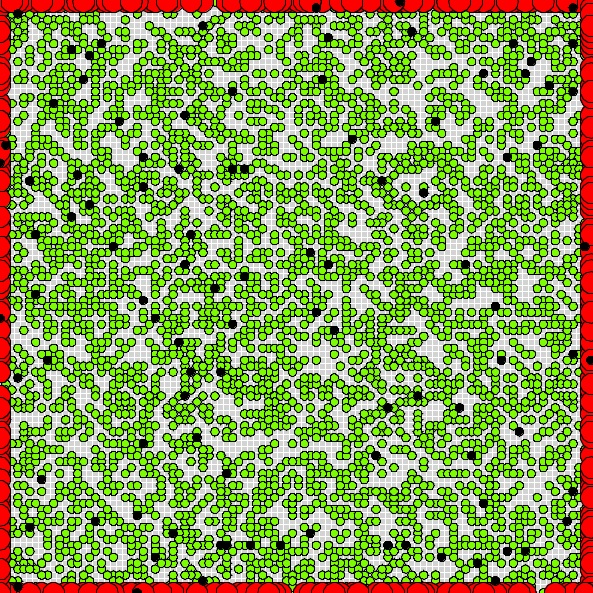
\includegraphics[scale=0.4]{kb2}
\end{center}
\caption{\textit{Hoa (màu đỏ) được phân bố tại biên của thửa ruộng}}
\end{figure}

\begin{figure}
\begin{center}
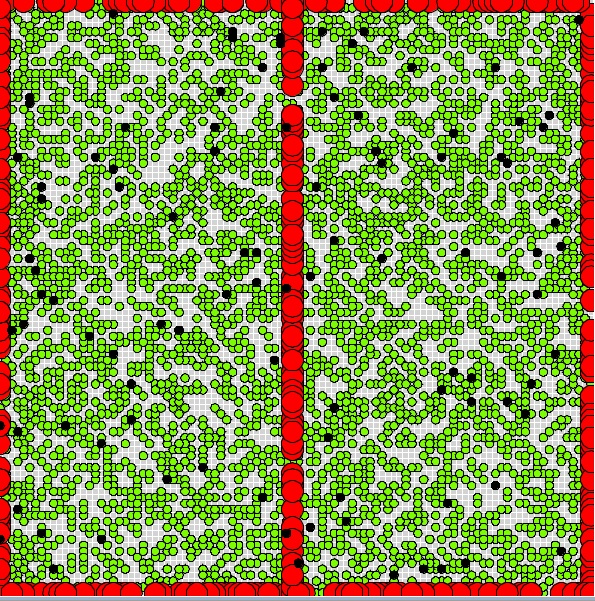
\includegraphics[scale=0.4]{kb3}
\end{center}
\caption{\textit{(Hoa (màu đỏ) được phân bố trên biên và một đoạn thẳng trung tuyến}}
\end{figure}
%h1: Hoa (màu đỏ) được phân bố theo các kịch bản khác nhau trên ruộng

\textit{Thiên địch}: Rầy nâu có một số loài  thiên địch có thể tiêu diệt được và được
ứng dụng như biện pháp sinh học phòng trừ rầy nâu. Cụ thể trong mô hình này, chúng tôi xét thiên địch là loài Nhện ăn thịt (Lycosa  pseudoannulata). Loài nhện này thường gặp rất 
nhiều trên ruộng lúa, chúng chủ động tấn công rầy rất nhanh. Một 
con nhện trưởng thành có thể ăn thịt từ 5-15 con rầy nâu mỗi 
ngày. Ngòai rầy nâu chúng còn tấn công nhiều loài sâu hại khác 
như  bướm của của các loài sâu thuộc Bộ cánh phấn...

\textit{Rầy nâu}: Số lượng rầy nâu $N_3$, rầy nâu được mô phỏng theo vòng đời của chúng. Số lượng rầy nâu thay đổi do tỉ lệ sinh  $r_3$, tỉ lệ chết theo thời gian  $\mu_3$ và sinh trưởng khi chích hút lúa hay bị thiên địch ăn thịt.

Vòng đời của rầy nâu kéo dài khoảng 25-28 ngày ở nhiệt độ $25-30^0C$, bao gồm ba giai đoạn sinh trưởng: trứng, con non và con trưởng thành. Sau khi trứng nở từ 5-7 ngày, con non trải qua năm giai đoạn trong vòng 12-14 ngày và phát triển thành con trưởng thành cánh ngắn hoặc cánh dài. Sự thay đổi sinh học này của rầy nâu tùy thuộc vào điều kiện thời tiết và môi trường từng địa phương [Mochida and Okada, 1979]. Các con trưởng thành cánh ngắn theo quy luật sẽ xuất hiện trước giai đoạn lúa làm đòng và đầu vụ thu hoạch, trong khi con trưởng thành cánh dài phát triển mạnh để di cư. Mỗi lần đẻ trứng, một con rầy cái trưởng thành cánh ngắn có thể sinh 300 trứng và 100 trứng với một con cánh dài trưởng thành [13].

%Nhiệt độ là nhân tố có ảnh hưởng nhất tới sự chuyển giữa giai đoạn sinh trưởng của %rầy nâu [Mochida and Okada, 1979]. Cụ thể được mô tả theo bảng 
Cụ thể, sự phát triển của rầy nâu theo thời gian liên tục tuân theo các phương trình mô tả trong Bảng 3.1. [13]
\begin{table}
\begin{tabular}{m{7cm} m{8cm}}
\hline
{Sự biến đổi} & \textit{Phương trình} \\ 
\hline
\textit{Số lượng trứng} & $E(t+1) = [E(t)-E'(t)+E1(t)]*R_e$ \\ 
\hline
\textit{Số lượng con non} & $N(t+1)=[N(t)-N'(t)+E'(t)*P_e]*R_n$ \\ 
\hline
\textit{Số lượng con trưởng thành} & $MS+ML+FMS+FML$ \\
\hline
\textit{Số lượng con trưởng thành đực cánh ngắn} & $MS(t+1)=[MS(t)-MS'(t)+N'(t)*P_n*S_a]*R_a$ \\
\hline
\textit{Số lượng con trưởng thành đực cánh dài} & $ML(t+1)=[ML(t)-ML'(t)+N'(t)*P_n*S_a]*R_a$ \\
\hline
\textit{Số lượng con trưởng thành cái cánh ngắn} & $FMS(t+1)=[FMS(t)-FMS'(t)+N'(t)*P_n*S_a]*R_a$ \\
\hline
\textit{Số lượng con trưởng thành cái cánh dài} & $FML(t+1)=[FML(t)-FML'(t)+N'(t)*P_n*S_a]*R_a$ \\
\hline
\textit{Số lượng trứng sinh ra (giai đoạn rầy trưởng thành đẻ trứng)} & $E1(t+1)=FMS*300+FML*100$ \\
\hline
\end{tabular}
\caption{\textit{Các hàm biểu thị sự phát triển của rầy nâu theo thời gian liên tục}}
\end{table}
 
{%\eqref{Hình 1}
%h1: Vòng đời rầy nâu và các nhân tố ảnh hưởng
%\begin{figure}%\label{Hình 1}
%\begin{center}
%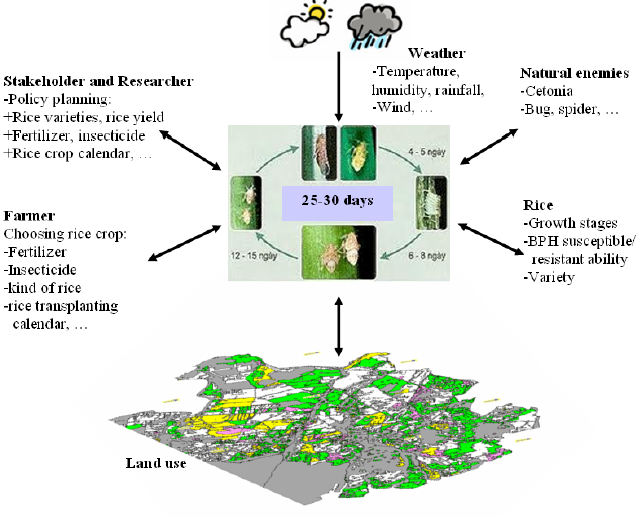
\includegraphics[scale=0.8]{ahg}
%\end{center}
%\caption{\textit{Vòng đời rầy nâu và các nhân tố ảnh hưởng \cite{nngv} }}
%\end{figure}}

\subsection*{Phạm vi}
Phạm vi không gian mô hình xét đến là trên một thửa ruộng. Phạm vi thời gian của mô hình là 120 ngày xét trên thang thời gian sinh trưởng của lúa, đơn vị thời gian là 0.5 ngày nghĩa là mỗi bước mô phỏng tương ứng với 0.5 ngày.

\section{Tiến trình và kế hoạch}

\textit{\indent Cây lúa}: Khi bắt đầu mô phỏng, lượng lúa được phân bố ngẫu nhiên trên ruộng và vị trí cố định cho đến lúc bị chết đi. Lúa sinh trưởng nhờ việc lấy khoáng từ vị trí nó. Lúa khi bước vào giai đoạn đẻ nhánh trong giai đoạn sinh trưởng (đủ tuổi) bắt đầu bị rầy tấn công. Thời điểm thường bắt đầu từ ngày thứ 45 trở đi \cite{sachhd2}. Rầy non cũng có khả năng hút nhựa lúa. Rầy nâu trưởng thành di chuyển theo hướng gió gặp lúa đủ tuổi, nó sẽ chích hút nhựa lúa, khiến lúa chết (xem Hình 3.3).

\textit{Hoa:} Khi bắt đầu mô phỏng, hoa được phân bố theo các kịch bản khác nhau (xem Hình 3.1 - 3.2) và giữ vị trí cố định trong cả quá trình mô phỏng. Hoa sinh trưởng nhờ việc lấy khoáng từ vị trí của nó. Nếu vị trí hoa và lúa nằm trong phạm vi đủ gần, chúng sẽ cạnh tranh khoáng chất với nhau. Rầy nâu trưởng thành di chuyển theo hướng gió nếu gặp thiên địch, khi đó rầy sẽ bị thiên địch ăn thịt, một phần xác rầy chết rơi xung quanh cây hoa và làm nguồn dinh dưỡng cho cây.

\textit{Thiên địch:} Thiên địch bị thu hút đến vùng có hoa, số lượng thiên địch sẽ tăng theo mỗi bước thời gian. Xét với loài nhện ăn thịt, chúng có vòng đời 30 ngày tương tự như rầy nâu. Khả năng sinh sản mỗi lần của một con nhện cái cũng có thể tới 300 trứng.

\textit{Rầy nâu:} Rầy nâu là loài côn trùng có chu kì phát triển theo kiểu biến thái không hoàn toàn, phải trải qua 3 pha phát dục: pha trứng, pha ấu trùng (rầy non) và pha trưởng thành. Vòng đời phát triển của rầy nâu được mô tả trong Hình 2.6. Trong điều kiện nhiệt độ $25-30^o C$, vòng đời rầy nâu thường từ 25-30 ngày: trứng phát triển thành rầy non từ 5-7 ngày, rầy non trưởng thành từ 12-14 ngày, sau đó đẻ trứng và chết đi \cite{sachhd1}. Rầy trưởng thành có hai loại: cánh dài và cánh ngắn. Rầy trưởng thành cánh dài xâm nhập vào ruộng lúa và đẻ trứng trên các bẹ lá hoặc ở các gân lá \cite{sachhd2}. Rầy non có màu trắng, các tuổi sau có màu vàng nâu \cite{sachhd2}. Rầy cánh dài thường xuất hiện vào giai đoạn đầu và giai đoạn lúa chín, di chuyển, phát tán. Rầy trưởng thành di chuyển 0.5 ngày/ lần. Phòng thí nghiệm Viện Khoa Học Kĩ Thuật Nông Nghiệp Miền Nam cho số liệu một trưởng thành cái của rầy nâu đẻ trung bình 150-400 trứng. Nuôi thí nghiệm ở Long An, mỗi trưởng thành cái đẻ 50-200 trứng. Tronh điều kiện vùng Hà Nội, một trưởng thành cái có khả năng đẻ 110 - 324 trứng \cite{sachhd1}.

%hình 3
\begin{figure}
\begin{center}
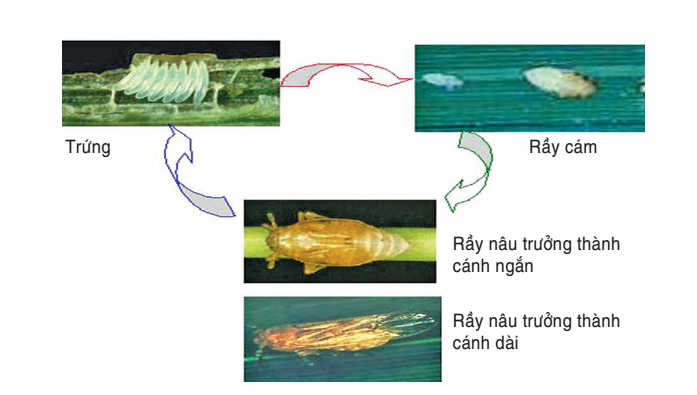
\includegraphics[scale=0.8]{vongdoiray}
\end{center}
\caption{\textit{Vòng đời phát triển của rầy nâu}}
\end{figure}

\textit{Lịch trình:} Khi bắt đầu mô phỏng, lúa và rầy được phân bố ngẫu nhiên trên các ô khoáng, hoa được phân bố ngẫu nhiên hay theo cách sắp xếp với số lượng ban đầu cụ thể. Tai mỗi bước thời gian của mô phỏng, lúa và hoa sinh trưởng nhờ việc lấy khoáng từ ô khoáng chất tại vị trí của chúng, đồng thời age của lúa, hoa và rầy đều tăng lên và energy của chúng mất đi một lượng cho sinh trưởng. Đến ngày 21, rầy trưởng thành và bắt đầu đẻ trứng và 7 ngày sau kết thúc vòng đời đầu tiên. Rầy sẽ lặp lại vòng đời theo chu kì 30 ngày. Đến ngày 45, lúa bước vào giai đoạn đẻ nhánh và bắt đầu bị rầy tấn công. Rầy trưởng thành di chuyển theo tốc độ và hướng gió, khi gặp và hút nhựa lúa khiến lúa chết. Nếu rầy di chuyển gặp hoa, nó sẽ bị thiên địch ăn thịt.

\section{Các khái niệm nền tảng}
\subsection{Các quy tắc cơ bản}
\indent Rầy di chuyển theo gió gặp lúa và hại lúa có thể theo cách trực tiếp là chích hút nhựa lúa hoặc gián tiếp môi giới truyền vi rút gây bệnh vàng lùn, lùn xoắn lá cho cây lúa. Cả hai cách đều khiến lúa không trổ bông được, năng suất giảm nghiêm trọng hay mất trắng \cite{tltk9, tltk10}.

\indent Rầy hút được nhựa lúa biến thành năng lượng để sống. Tuy nhiên, nếu rầy di chuyển tới vùng có hoa, gặp thiên địch, nó sẽ bị thiên địch ăn thịt và một phần xác rơi xuống làm dưỡng chất cho hoa.

\indent Các thực thể trong mô hình là lúa, hoa, thiên địch và rầy mất năng lượng theo từng bước thời gian do sinh trưởng ngoài ra còn mất năng lượng do di chuyển (thiên địch và rầy nâu).

\subsection{Sự nổi bật}
Sự nổi bật hay kết quả đầu ra ta quan tâm nhất ở đây là ảnh hưởng của phân bố không gian của hoa trên ruộng tới sự sinh trưởng và hại lúa của rầy nâu, điều chưa đoán biết được trong các điều kiện đầu vào ban đầu của mô hình và sự thay đổi của môi trường.

\subsection{Mục tiêu}
Mục tiêu của mô hình là xem xét sự khác nhau của mật độ sinh trưởng và hại lúa của rầy nâu cùng với sự phát triển của lúa với những kịch bản phân bố vị trí không gian của hoa khác nhau trên ruộng lúa (Hình 3.1 - 3.2). Mục tiêu này được rút ra từ việc ghi nhận sự phát triển về số lượng rầy nâu cũng như số lượng phát triển của lúa theo thời gian.

\subsection{Tương tác}
Tương tác giữa rầy và lúa là việc rầy hút nhựa lúa, khiến lúa chết, ảnh hưởng tới năng suất. Hoa thu hút thiên địch của rầy tới vùng có trồng hoa, nên rầy sẽ bị thiên địch ăn thịt khi di chuyển tới vùng có hoa, ảnh hưởng tới mật độ rầy. Đồng thời, vùng hoa sẽ cản bước di chuyển của rầy. Lúa và hoa có tương tác cạnh tranh khoáng trong đất để sinh trưởng.

\subsection{Quan sát}
Chúng tôi ghi nhận số lượng rầy nâu và lúa trên ruộng trước và sau mỗi ngày. Từ đó thu được số liệu về mật độ rầy và số lúa chết mỗi ngày.

\section{Khởi tạo}
khởi tạo mô phỏng với 300000 cây lúa, 300 con rầy được phân bố ngẫu nhiên trên ruộng. 1000 cây hoa cũng được khởi tạo khi bắt đầu mô phỏng và được phân bố tương ứng với 2 kịch bản phân bố không gian: (a) Hoa phân bố tại biên của thửa ruộng (b) Hoa phân bố trên biên và một đoạn thẳng trung tuyến (Hình 3.1 - 3.2).

\section{Dữ liệu đầu vào}
Trạng thái rầy di chuyển được mô phỏng phụ thuộc vào hướng và tốc độ gió, là các điều kiện môi trường cần dữ liệu đầu vào.

\section{Mô hình con}
\textit{Rầy hại lúa:} Rầy ở giai đoạn con non cũng đã có khả năng hút nhựa khiến lúa mất đạm, khô mà chết. Rầy hại lúa khi nó bước vào giai đoạn trưởng thành (có thể di chuyển) và lúa vào giai đoạn đẻ nhánh (đủ tuổi) không chỉ hút đạm mà còn thêm khả năng truyền virut gây bệnh (vàng lùn, lùn xoắn lá,...).

\textit{Hoa ăn rầy:} Khi di chuyển, nếu rầy theo hướng gió di chuyển tới vị trí vùng có hoa, nếu gặp thiên địch, rầy sẽ bị ăn thịt.

\textit{Sự cạnh tranh khoáng chất:} Lúa và hoa cạnh tranh khoáng tại vị trí của mình để sinh trưởng.

Từ đó, chúng tôi đề xuất mô hình phương trình (Equation-based model viết tắt là EBM) thể hiện sự thay đổi mật độ các loài trong mô hình dựa trên cá thể (Agent-based model viết tắt là ABM) đang xét

\begin{flushleft}
\begin{equation}\label{1}
\dfrac{d N_1}{dt} = r_1 N_1 - \mu_1 N_1 - a_{12} N_1  N_2 - b_{31} N_1 N_3
\end{equation}
\begin{equation}\label{2}
\dfrac{d N_2}{dt} = r_2 N_2 - \mu_2  N_2 - a_{21} N_2 N_1 + b_{23} e_{23} N_2 N_3
\end{equation}
\begin{equation}\label{3}
\dfrac{d N_3}{dt} = r_3 N_3 - \mu_3  N_3 + b_{31} e_{31} N_3 N_1 - b_{23} N_2 N_3
\end{equation}
\end{flushleft}

\indent(1) Lúa sinh trưởng tự nhiên với tỉ lệ sinh $r_1$, bị chết theo tỉ lệ chết $\mu_1$, cạnh tranh khoáng với hoa theo hệ số cạnh tranh $a_{12}$  và chết do bị rầy ăn với hệ số bắt mồi $b_{31}$.

(2) Hoa sinh trưởng tự nhiên với tỉ lệ sinh $r_2$, bị chết theo tỉ lệ chết $\mu_2$, sinh trưởng nhờ xác rầy chết theo tỉ lệ chuyển hóa $b_{23} e_{23}$ và cạnh tranh khoáng với hoa theo hệ số cạnh tranh $a_{21}$.

(3) Rầy nâu sinh trưởng tự nhiên với tỉ lệ sinh $r_3$, bị chết theo tỉ lệ chết $\mu_3$, sinh trưởng nhờ thức ăn ăn được từ lúa theo tỉ lệ chuyển hóa $b_{31} e_{31}$ và chết do bị hoa ăn với hệ số bắt mồi $b_{23}$.

\section*{Kết luận}
Trong chương 3, chúng tôi đã mô tả mô hình đa tác tử của rầy nâu và lúa với phân bố hoa thu hút thiên địch của rầy theo giao thức chuẩn ODD. Với các trạng thái và hành vi của các thực thể trong mô hình đã được mô tả, chúng tôi thực hiện xây dựng chương trình mô phỏng cho mô hình đang xét bằng phần mềm GAMA. Trong chương 4, chúng tôi sẽ trình bày việc xây dựng chương trình mô phỏng của mô hình và các kết quả thu được từ chương trình mô phỏng.

\newpage
\chapter{Kết quả nghiên cứu và thảo luận}
\section{Các thí nghiệm mô phỏng}
\subsection{Thí nghiệm 1}
Mô phỏng được xây dựng trong môi trường grid phạm vi $ 100 \times 100$. Khởi tạo mô phỏng với 30000 cây lúa, 1000 cây hoa, 700 con nhện (thiên địch) và 300 con rầy.

Mỗi cây lúa được mô phỏng như một cá thể của loài lúa, gồm các thuộc tính:
\begin{itemize}
\item location: ô vị trí sinh trưởng, cố định trong suốt quá trình mô phỏng.
\item energy: năng lượng nội tại, cây lúa chết khi energy <=0.
\item age: tuổi lúa, sử dụng để xác định thời điểm mà lúa bắt đầu bị rầy tấn công.
\end{itemize}

Mỗi cây hoa được mô phỏng như một cá thể của loài hoa, gồm các thuộc tính:
\begin{itemize}
\item location: ô vị trí sinh trưởng, cố định trong suốt quá trình mô phỏng.
\item energy: năng lượng nội tại, cây hoa cũng chết khi energy <=0.
\end{itemize}

Mỗi con nhện được mô phỏng như một cá thể của loài thiên địch, gồm các thuộc tính:
\begin{itemize}
\item location: ô xác định vị trí cá thể.
\item energy: năng lượng nội tại của cá thể, nhện chết khi energy <=0. Năng lượng của nhện tăng lên nếu nó bắt và ăn thịt được rầy.
\item age: tuổi nhện, sử dụng để xác định giai đoạn vòng đời sinh trưởng của nhện.
\end{itemize}

Mỗi con rầy được mô phỏng như một cá thể của loài rầy, gồm các thuộc tính:
\begin{itemize}
\item location: ô vị trí rầy
\item energy: năng lượng nội tại của cá thể rầy, rầy chết khi energy <=0. Năng lượng của rầy tăng lên nếu nó di chuyển đến vị trí có lúa và ăn lúa, khiến lúa chết.
\item age: tuổi rầy, sử dụng để xác định rầy thuộc pha nào trong vòng đời sinh trưởng.
\end{itemize}

Chương trình mô phỏng dưới dạng giải thuật sau:

\textit{\textbf{Đầu vào:}} Dữ liệu đầu vào về thời tiết: hướng, vận tốc gió; Số lượng các loài ban đầu; Tham số hành vi của từng loài: tỉ lệ chuyển hóa, năng lượng sinh sản, năng lượng mất do sinh trưởng.

\textbf{\textit{Đầu ra:}} Đồ thị thể hiện số lượng các loài biến đổi trong mô hình theo mỗi bước mô phỏng.
%\Khung{.9\textwidth}{
\begin{center}
\small{
\begin{verbatim}
foreach time_step from 1 to time=120#day do
	foreach agent is in [lua] do
	update lua age;
	foreach agent is in [ray] do
	update  age;
	if age>=30 then do die;
	if age>=7 then
	get wind_dir, wind_speed of current time step;
	do wind_move and eat_rice;
	if age >=21 then do reproduce;
	foreach agent is in [thien_dich]
	update hoa location
	do migrate and eat_ray;
\end{verbatim}
}
\end{center}

Quá trình mô phỏng được chạy với các giá trị ban đầu khởi tạo của các loài như nhau, chương trình chạy 50 lần mô phỏng để lấy số liệu phát triển của ba loài xét trong mô hinh trung bình tương ứng với mỗi kịch bản (a) Hoa phân bố tại biên của thửa ruộng (b) Hoa phân bố trên biên và một đoạn thẳng trung tuyến. Hình 4.1 và Hình 4.2 mô tả đồ thị theo thời gian của các loài tương ứng với mỗi kịch bản. Hình 4.3 là đồ thị biểu diễn sự phát triển của rầy với các kịch bản đang xét trong một trường hợp chạy mô phỏng.

\begin{figure}%\label{Hình 1}
\begin{center}
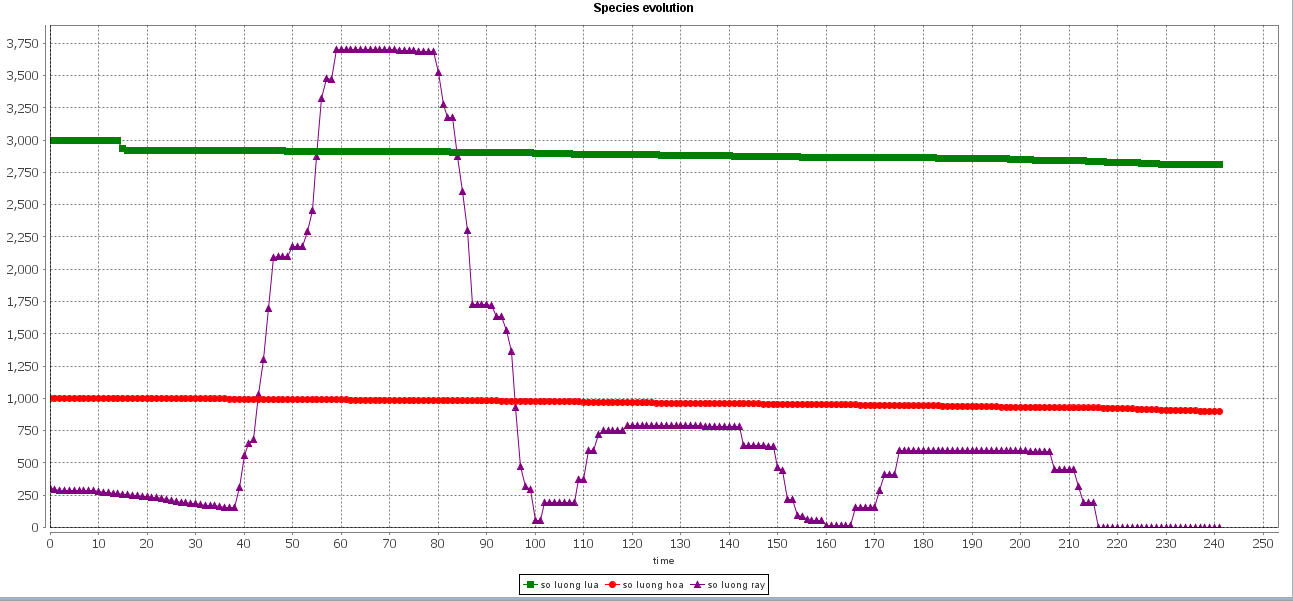
\includegraphics[scale=0.4]{kb2gr}
\end{center}
\caption{\textit{Sự phát triển của các loài theo thời gian trong một lần chạy mô phỏng (kịch bản (a))}}
\end{figure}

\begin{figure}%\label{Hình 1}
\begin{center}
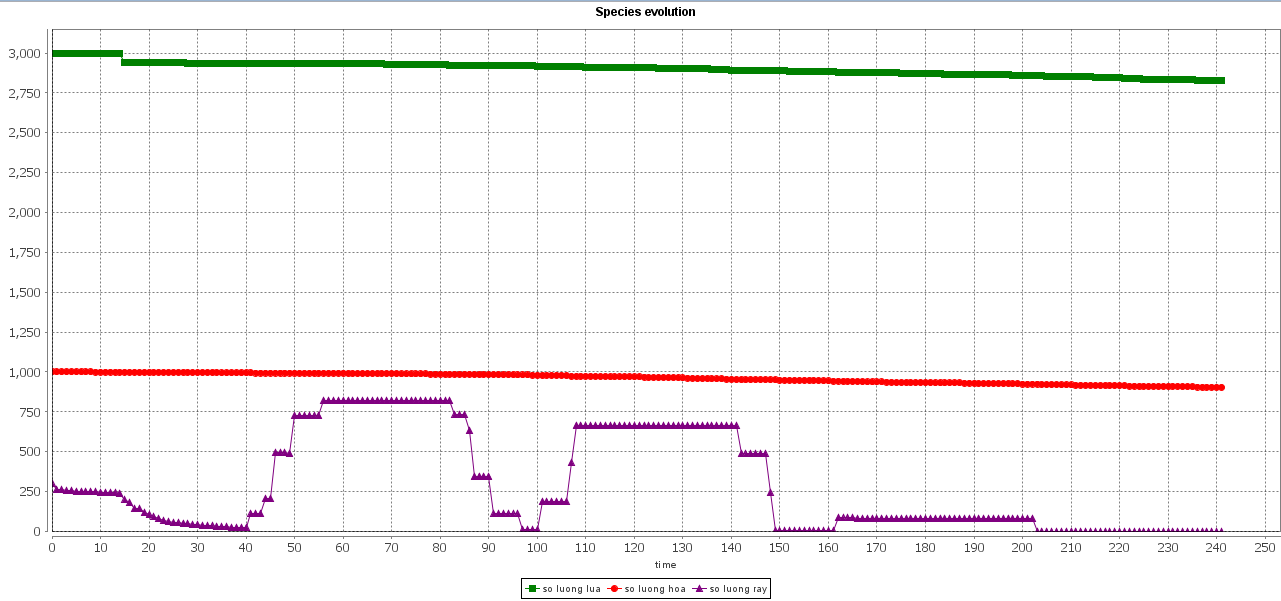
\includegraphics[scale=0.4]{kb3gr}
\end{center}
\caption{\textit{Sự phát triển của các loài theo thời gian trong một lần chạy mô phỏng (kịch bản (b)}) }
\end{figure}

\begin{figure}%\label{Hình 1}
\begin{center}
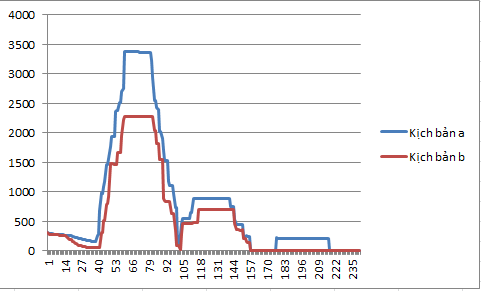
\includegraphics[scale=1]{2kb}
\end{center}
\caption{\small Sự phát triển của rầy theo thang thời gian tương ứng với hai kịch bản }
\end{figure}

\subsection{Thí nghiệm 2}
Mở rộng mô hình với hai kịch bản xét trên 9 thửa ruộng (xem Hình 4.4 - 4.5). Khởi tạo mô phỏng với 30000 cây lúa, 1000 cây hoa, 700 con nhện (thiên địch) ở mỗi thửa ruộng. Khởi tạo 300 con rầy ban đầu chỉ tại thửa ruộng thứ nhất.
\begin{figure}%\label{Hình 1}
\begin{minipage}[b]{0.5\linewidth}
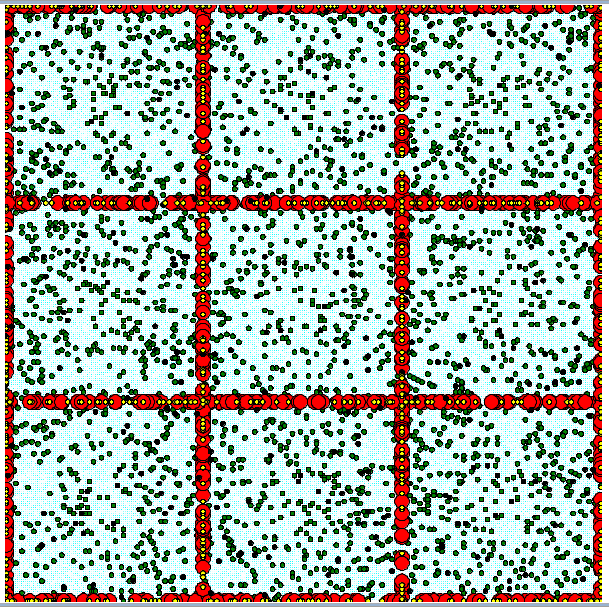
\includegraphics[scale=0.4]{kb91}
\caption{\textit{ Mô phỏng mở rộng trên 9 thửa ruộng tương ứng với kịch bản (a)}}
\end{minipage}
\hspace{0.5cm}
\begin{minipage}[b]{0.5\linewidth}
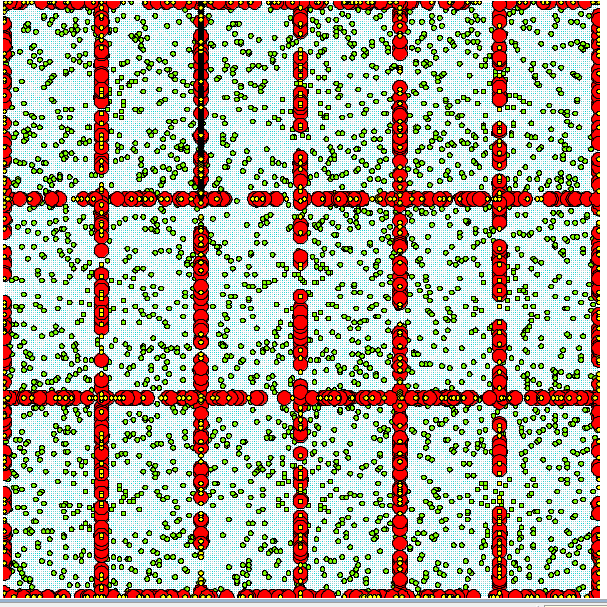
\includegraphics[scale=0.4]{kb92}
\caption{ \textit{Mô phỏng mở rộng trên 9 thửa ruộng tương ứng với kịch bản (b)} }
\end{minipage}
\end{figure}


\begin{figure}%\label{Hình 1}
\begin{center}
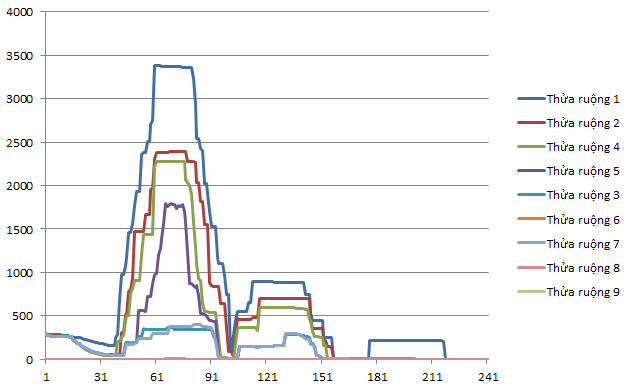
\includegraphics[scale=0.8]{kq9a}
\end{center}
\caption{ \textit{Số lượng rầy nâu trên 9 thửa ruộng tương ứng với kịch bản (a)}}
\end{figure}

\begin{figure}%\label{Hình 1}
\begin{center}
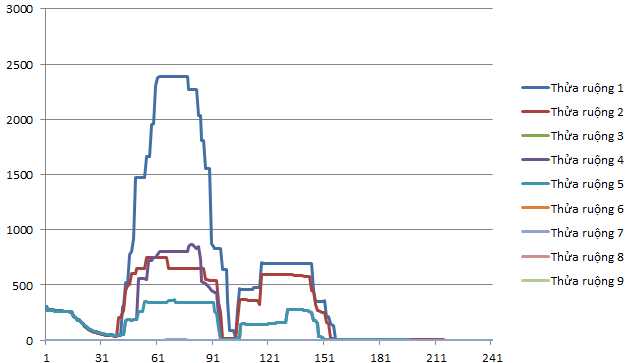
\includegraphics[scale=0.8]{kq9b}
\end{center}
\caption{\textit{Số lượng rầy nâu trên 9 thửa ruộng tương ứng với kịch bản (b)} }
\end{figure}

%\begin{figure}%\label{Hình 1}
%\begin{center}
%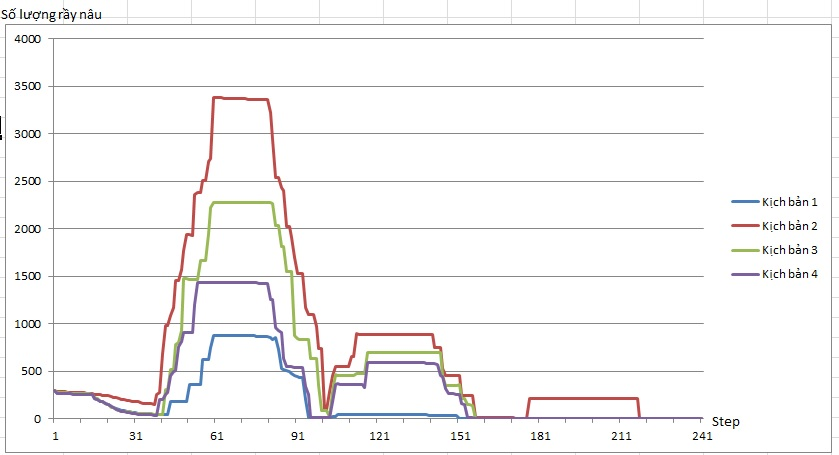
\includegraphics[scale=0.6]{4kbrn}
%\end{center}
%\caption{\small Sự phát triển của rầy theo thang thời gian tương ứng tăng lượng rầy ban đầu }
%\end{figure}
%Mở rộng mô hình xét trên 9 thửa ruộng, với cùng lượng rầy ban đầu chỉ trong một thửa, kết quả trung bình đạt được như sau.\\


\section{Các kết quả đạt được}
Từ đồ thị, tôi đưa ra so sánh lượng rầy phát triển trong cả quá trình mô phỏng giữa hai kịch bản như sau: Mật độ rầy giảm đi trong kịch bản (b) so với kịch bản (a). Việc phân bố hoa theo cả đường biên và đường trung tuyến có kết quả hạn chế sự phát triển rầy nâu tốt hơn so với việc chỉ phân bố hoa trên biên.
%Mật độ hoa trên ruộng cũng có ảnh hưởng đến sự phát triển của rầy. Cụ thể, số liệu được thể hiện trong Hình 3.4 và Hình 3.5. Trong cả hai kịch bản, khi số lượng hoa tăng, lượng rầy có thay đổi theo chiều hướng giảm.

Với trường hợp mở rộng mô hình xét trên 9 thửa ruộng, với cùng lượng rầy ban đầu chỉ trong một thửa, trường hợp trồng hoa trên biên và một đường trung tuyến vẫn cho kết quả ngăn chặn sự phát triển của rầy tốt hơn. Hơn thế nữa, việc trồng hoa trên biên và đường trung tuyến còn có tác dụng ngăn cản bước di chuyển của rầy. Kịch bản (a) mở rộng với phạm vi 9 thửa ruộng, rầy lây lan qua phạm vi 6 thửa (xem Hình 4.6). Kịch bản (b) mở rộng cho kết quả tốt hơn, rầy hầu như lây lan chỉ qua phạm vi đến 4 thửa là đã bị ngăn chặn hoàn toàn (xem Hình 4.7). 
\newpage

\chapter{Kết luận}
Trong đồ án này, chúng tôi đã giới thiệu và trình bày một số khái niệm cơ bản về mô hình, chu trình phát triển mô hình và mô hình hóa dựa trên cá thể. Chúng tôi cũng giới thiệu tổng quan về giao thức ODD và sử dụng nó để mô tả và xây dựng mô hình rầy nâu hại lúa, từ đó đưa ra kết luận ảnh hưởng phân bố không gian của hoa thu hút thiên địch lên sự phát triển của rầy nâu ứng với hai kịch bản. Các kết quả thu được của đồ án:
\begin{itemize}
\item Xây dựng và mô hình hóa dựa trên cá thể mô hình rầy nâu hại lúa.
\item Mô phỏng sự phát triển và lây lan của rầy nâu ứng với hai kịch bản phân bố không gian của hoa thu hút thiên địch rầy nâu trên GAMA.
\item So sánh sự phát triển của rầy nâu trên ruộng giữa hai kịch bản phân bố không gian của hoa.
\item Kết luận về mối liên hệ giữa phân bố không gian của hoa với sự phát triển và lây lan của rầy nâu: Xét trên một thửa ruộng và mô hình mở rộng với 9 thửa ruộng, việc trồng hoa theo đường biên và một trung tuyến có kết quả diệt và ngăn chặn rầy tốt hơn so với chỉ trồng trên biên với cùng số lượng hoa đó
\end{itemize} 

Hướng phát triển tiếp theo chúng tôi muốn mở rộng mô phỏng trong không gian lớn với số lượng cá thể lúa, hoa, rầy tới vài trăm triệu cá thể trên nhiều thửa ruộng của một xã, huyện thậm chí là một vài tỉnh để từ đó giúp người nông dân đưa ra quyết định tốt hơn trong việc diệt trừ rầy nâu hại lúa. Hơn nữa, chúng tôi sẽ áp dụng mô hình trên môi trường thực tế dựa vào bản đồ thông tin địa lý (Geographic Information system viết tắt là \textit{GIS}) của các vùng trồng lúa ở Việt Nam.\\
\newpage
\addcontentsline{toc}{chapter}{{Danh mục công trình công bố của tác giả}}
\chapter*{Danh mục công trình công bố của tác giả}
\begin{flushleft}
\quad $[1]$\ Vũ Thu Thảo, Nguyễn Ngọc Doanh, Nguyễn Nhị Gia Vinh, Nguyễn Thị\\\quad \quad \   Ngọc
Anh, \textit{"Mô hình hóa ảnh hưởng phân bố không gian của hoa diệt rầy\\ \quad \quad \  tới
sự phát triển của rầy nâu hại lúa"}, Tạp chí Khoa học và Công nghệ -\\\quad \quad \  Đại học Thái Nguyên, 2015, pp.119-123.\\
\end{flushleft}
\newpage
\addcontentsline{toc}{chapter}{{Tài liệu tham khảo}}
\bibliographystyle{amsplain}
\thispagestyle{empty}
\bibliography{science}

Bài toán: Với một dãy quan sát $O = O_1, O_2, ..., O_T$, và mô hình $\lambda$, ta phải tìm ra dãy trạng thái ẩn $Q = q_1, q_2, ..., q_T$ hợp lí nhất.\\
Với mỗi trạng thái ẩn $q_t$, ta đặt:
\[\gamma_t(i) = P(q_t = S_i|O, \lambda)\]
Đây là xác suất hệ thống ở trạng thái $S_i$ tại thời điểm $t$, với điều kiện biết được dãy quan sát $O$ và mô hình $\lambda$.\\
Theo thuật toán Forward-Backward, ta đã có:
\[\alpha_t(i) = P(O_1, O_2, ..., O_t, q_t=S_i|\lambda)\]
\[\beta_t(i) = P(O_{t+1}, O_{t+2}, ..., O_T| q_t=S_i, \lambda)\]
Theo tiêu chuẩn d-separation, ta có:
\[p(O_1, O_2, ..., O_T|q_t=S_i, \lambda) = p(O_1, O_2, ..., O_t|q_t=S_i, \lambda)
.p(O_{t+1}, O_{t+2}, ..., O_T| q_t=S_i, \lambda)\]
Mặt khác, theo định lý Bayes:
\[P(q_t=S_i|O, \lambda) = \frac{P(O|q_t=S_i, \lambda).P(q_t=S_i|\lambda)}{P(O|\lambda)}\]
Do đó
\[ \gamma_t(i)=\frac{\alpha_t(i)\beta_t(i)}{P(O|\lambda)}=\frac{\alpha_t(i)\beta_t(i)}{\sum_{i=1}^{N}\alpha_t(i)\beta_t(i)}\]
Với $\gamma_t(i)$, ta có thể dễ dàng tìm được trạng thái hợp lí nhất $q_t$ tại thời điểm t
\[q_t = \argmax_{1\le i \le N} \gamma_t(i)\]
Tuy nhiên, kết quả trên chỉ cho ta trạng thái hợp lí nhất tại một thời điểm nhất định. Ta cần phải tìm ra dãy trạng thái ẩn phù hợp nhất với dãy quan sát có được.\\
Ta định nghĩa:
\[\delta_t(i) = \max_{q_1, q_2, ..., q_{t-1}}P(q_1, q_2, ..., q_t=i, O_1, O_2, ..., O_t|\lambda)\]
$\delta_t(i)$ có thể được hiểu là xác suất lớn nhất cho đến thời điểm t của dãy các trạng thái ẩn ứng với t quan sát đầu tiên, sao cho tại t hệ thống ở trạng thái $S_i$.\\
Dễ thấy
\[\delta_{t+1}(i) = \max_i(\delta_t(i)a_{ij}).b_j(O_{t+1})\]
Sau mỗi bước tính toán, ta lưu lại $\argmax_i(\delta_t(i)a_{ij})$.\\
Từ đây, việc tìm ra dãy trạng thái phù hợp nhất có thể thực hiện bằng cách lần lượt tính các giá trị $\delta_1(i), \delta_2(i), ...$ cho đến $\delta_T(i)$, sau đó thực hiện truy vết, tìm ra các giá trị $q_i$. Đây chính là tư tưởng của thuật toán Viterbi.\\
Cụ thể hơn, thuật toán gồm các bước sau
\begin{itemize}
\item{Bước 1}. Bước khởi tạo
\[\delta_1(i) = \pi_i b_i(O_1), 1 \le i \le N\]
\[\Psi_1(i) = 0\]
\item{Bước 2}. Bước đệ quy
\[\delta_t(j) = \max_{1\le i \le N}(\delta_{t-1}(i)a_{ij})b_j(O_t), 2 \le t \le T, 1 \le j \le N\]
\[\Psi_t(j) = \argmax_{1\le i \le N}(\delta_{t-1}(i)a_{ij}), 2 \le t \le T, 1 \le j \le N\]
\item{Bước 3}. Bước dừng
\[P^* = \max_{1 \le i \le N} (\delta_T(i))\]
\[q_T^* = \argmax_{1 \le i \le N} (\delta_T(i))\]
\item{Bước 4}. Bước truy vết
\[q_t^* = \Psi_{t+1}(q_{t+1}^*), t = T-1, T-2, ..., 1\]
\end{itemize}
\end{document}